\documentclass[a4paper]{article}
\usepackage{tikz}
\usepackage{geometry}
\usepackage{graphicx}
\usepackage{natbib}
\usepackage{amsmath}
\usepackage{amssymb}
\usepackage{amsthm}
\usepackage{paralist}
\usepackage{epstopdf}
\usepackage{tabularx}
\usepackage{longtable}
\usepackage{multirow}
\usepackage{multicol}
\usepackage[hidelinks]{hyperref}
\usepackage{fancyvrb}
\usepackage{algorithm}
\usepackage{algorithmic}
\usepackage{float}
\usepackage{paralist}
%\usepackage[svgname]{xcolor}
\usepackage{enumerate}
\usepackage{array}
\usepackage{times}
\usepackage{url}
\usepackage{fancyhdr}
\usepackage{comment}
\usepackage{environ}
\usepackage{times}
\usepackage{textcomp}
\usepackage{caption}
\usepackage{bbm}


\urlstyle{rm}

\setlength\parindent{0pt} % Removes all indentation from paragraphs
\theoremstyle{definition}
\newtheorem{definition}{Definition}[]
\newtheorem{conjecture}{Conjecture}[]
\newtheorem{example}{Example}[]
\newtheorem{theorem}{Theorem}[]
\newtheorem{lemma}{Lemma}
\newtheorem{proposition}{Proposition}
\newtheorem{corollary}{Corollary}

\floatname{algorithm}{Procedure}
\renewcommand{\algorithmicrequire}{\textbf{Input:}}
\renewcommand{\algorithmicensure}{\textbf{Output:}}
\newcommand{\abs}[1]{\lvert#1\rvert}
\newcommand{\norm}[1]{\lVert#1\rVert}
\newcommand{\RR}{\mathbb{R}}
\newcommand{\CC}{\mathbb{C}}
\newcommand{\Nat}{\mathbb{N}}
\newcommand{\br}[1]{\{#1\}}
\DeclareMathOperator*{\argmin}{arg\,min}
\DeclareMathOperator*{\argmax}{arg\,max}
\renewcommand{\qedsymbol}{$\blacksquare$}

\definecolor{dkgreen}{rgb}{0,0.6,0}
\definecolor{gray}{rgb}{0.5,0.5,0.5}
\definecolor{mauve}{rgb}{0.58,0,0.82}

\definecolor{C0}{HTML}{1F77B4}
\definecolor{C1}{HTML}{FF7F0E}
\definecolor{C2}{HTML}{2ca02c}
\definecolor{C3}{HTML}{d62728}
\definecolor{C4}{HTML}{9467bd}
\definecolor{C5}{HTML}{8c564b}
\definecolor{C6}{HTML}{e377c2}
\definecolor{C7}{HTML}{7F7F7F}
\definecolor{C8}{HTML}{bcbd22}
\definecolor{C9}{HTML}{17BECF}

\newcommand{\Var}{\mathrm{Var}}
\newcommand{\Cov}{\mathrm{Cov}}
\newcommand{\sgn}{\mathrm{sgn}}

\newcommand{\vc}[1]{\mathbf{#1}}
\newcommand{\xv}{\vc{x}}
\newcommand{\Sigmav}{\vc{\Sigma}}
\newcommand{\alphav}{\vc{\alpha}}
\newcommand{\muv}{\vc{\mu}}

\newcommand{\red}[1]{\textcolor{red}{#1}}

\def\x{\mathbf x}
\def\y{\mathbf y}
\def\w{\mathbf w}
\def\v{\mathbf v}
\def\E{\mathbb E}
\def\R{\mathbb R}
\def\V{\mathbb V}
\def\ind{\mathbbm 1}
\renewcommand\vec[1]{\mathbf{#1}}
% TO SHOW SOLUTIONS, include following (else comment out):
\newenvironment{soln}{
    \leavevmode\color{blue}\ignorespaces
}{}


\hypersetup{
%    colorlinks,
    linkcolor={red!50!black},
    citecolor={blue!50!black},
    urlcolor={blue!80!black}
}

\geometry{
  top=1in,            % <-- you want to adjust this
  inner=1in,
  outer=1in,
  bottom=1in,
  headheight=3em,       % <-- and this
  headsep=2em,          % <-- and this
  footskip=3em,
}


\pagestyle{fancyplain}
\lhead{\fancyplain{}{Homework 6}}
\rhead{\fancyplain{}{CS 760 Machine Learning}}
\cfoot{\thepage}

\title{\textsc{Homework 7}} % Title

%%% NOTE:  Replace 'NAME HERE' etc., and delete any "\red{}" wrappers (so it won't show up as red)

\author{
\red{$>>$NAME HERE$<<$} \\
\red{$>>$ID HERE$<<$}\\
} 

\date{}

\begin{document}

\maketitle 


\textbf{Instructions:} 
You can choose any programming language as long as you implement the algorithm from scratch. Use this latex file as a template to develop your homework.
Submit your homework on time as a single pdf file to Canvas.
Please check Piazza for updates about the homework.\\


\section{ Principal Component Analysis [60 pts] 
}
Download {\tt three.txt} and {\tt eight.txt}. Each has $200$ handwritten digits. Each line is for a digit, vectorized from a $16\times 16$ grayscale image.
\begin{enumerate}
    \item  (10 pts) Each line has 256 numbers: They are pixel values ($0$=black, $255$=white) vectorized from the image as the first column (top-down), the second column, and so on. Visualize the two grayscale images corresponding to the first line in {\tt three.txt} and the first line in {\tt eight.txt}. 
\item (10 pts) Putting the two data files together (three first, eight next) to form an $n\times D$ matrix $\vec X$ where $n = 400$ digits and $D = 256$ pixels. Note we use $n \times D$ size for $\vec X$ instead of $D \times n$ to be consistent with the convention in linear regression. The $i$-th row of $X$ is $\vec x_i^\top$, where $\vec x_i\in\R^D$ is the $i$-th image in the 
combined data set. Compute the sample mean $\vec y=\frac{1}{n}\sum_{i=1}^n \vec x_i$. Visualize $\vec y$ as a $16\times 16$ grayscale image. 
\item (10 pts) Center $\vec X$ using $\vec y$ above. Then form the sample covariance matrix $\vec S=\frac{\vec X^\top \vec X}{n-1}$ Show the $5\times 5$ submatrix $\vec S(1\ldots 5,1\ldots 5)$.

\item (10 pts) Use appropriate software to compute the two largest eigenvalues $\lambda_1\geq \lambda_2$ and the corresponding eigenvectors $\vec v^1,\vec v^2$ of $\vec S$. For example, in Matlab one can use {\tt eigs(S,2)}. Show the value of $\lambda_1,\lambda_2$. Visualize $\vec v^1,\vec v^2$  as two $16\times 16$ grayscale images. Hint: Their elements will not be in $[0, 255]$, but you can shift and scale them appropriately. It is best if you can show an accompanying 'colorbar' that maps the grayscale to values. 
\item (10 pts) Now we project (the centered) $\vec X$ down to the two PCA directions. Let $\vec V = [\vec v^1\; \vec v^2]$ be the $D\times 2$ matrix. The projection is simply $\vec X\vec V$. Show the resulting two coordinates for the first line in {\tt three.txt} and the first line in {\tt eight.txt}, respectively. 
\item (10 pts) Now plot the 2D point cloud of the 400 digits after projection. For visual interest, color the points in {\tt three.txt} red and the points in {\tt eight.txt} blue. But keep in mind that PCA is an unsupervised learning method, and it does not know such class labels. 
\end{enumerate}

	\section{Directed Graphical Model [20 points]}
	Consider the directed graphical model (aka Bayesian network) in Figure~\ref{fig:bn}.
	\begin{figure}[H]
		\centering
		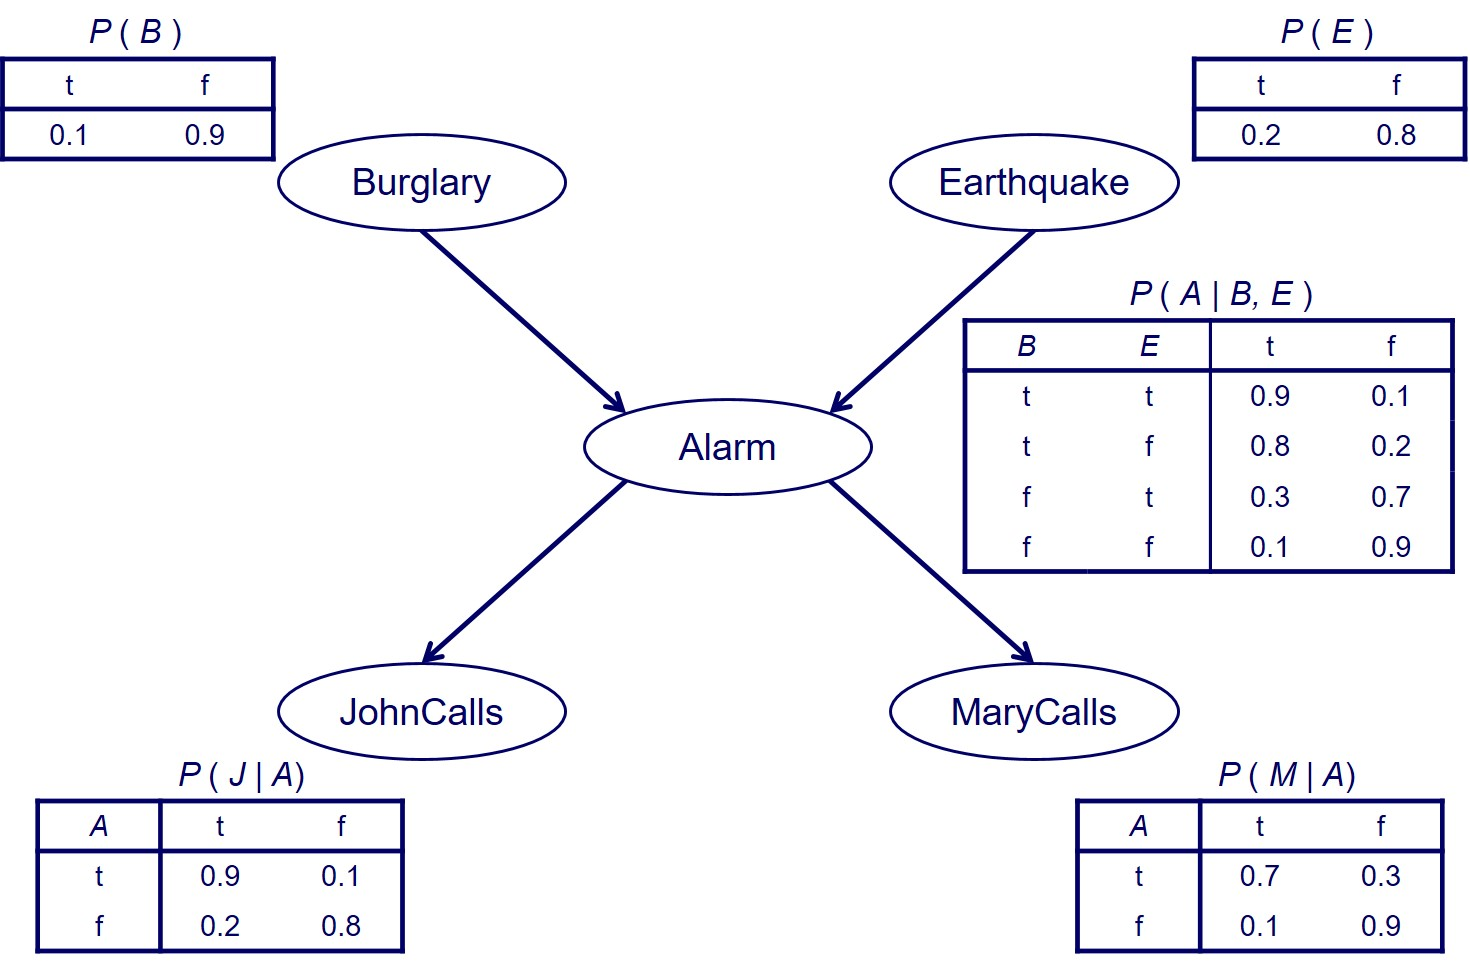
\includegraphics[width=0.8\textwidth]{BN.jpg}
		\caption{A Bayesian Network example.}
		\label{fig:bn}
	\end{figure}
	Compute $\mathbb{P}(B=t \mid E=f,J=t,M=t)$ and $\mathbb{P}(B=t \mid E=t,J=t,M=t)$.
	These are the conditional probabilities of a burglar in your house (yikes!) when both of your neighbors John and Mary call you and say they hear an alarm in your house, but without or with an earthquake also going on in that area (what a busy day), respectively.
	
	
\end{document}
